\documentclass[thesis.tex]{subfiles}
\def\x{\mathbf{x}}
\def\p{\mathbf{p}}
\def\c{\mathbf{c}}
\begin{document}
\chapter{Proposed descriptor}
%
Our proposed descriptor consists of weighted smooth histograms computed at several \textit{cells} arranged in a grid. We define the cell histogram $H_j$ as
%
\begin{align}
H_j(f_i) = \int F(\x) P (\x) A_j (\x) B(f_i, \x; f) \,\text{d} \x
\end{align}
%
where
%
\begin{itemize}
\item[] $f_i$ is a bin center,
\item[] $f$ is a value function defining the bin domain,
\item[] $F$ is a magnitude function,
\item[] $P$ is a center aperture function,
\item[] $A_j$ is a cell aperture function, and
\item[] $B$ is a binning aperture function.
\end{itemize}
%
Note that this definition is similar to the galaxy descriptor \cite{pedersen2013shape}, except we consider several histograms with their own aperture functions $A_j$ and add the additional center aperture function $P$. The descriptor $D$ is constructed by concatenating all $n$ bin values of all $m$ cell histograms:
%
\begin{align}
D = \Bigl( \left(H_1(f_1) \cdots H_1(f_n)\right) \cdots (H_m(f_1) \cdots H_m(f_n)) \Bigr)
\end{align}
%
The five functions above can be seen as the components that make up our descriptor, and we consider different choices for each.
%
\section{Value and magnitude functions}
%
The choice of value and magnitude functions are closely connected, as we wish the magnitude function to weight the histogram values according to their importance for the local image structure. The by far most common choice in literature \cite{lowe2004distinctive,ke2004pca,mikolajczyk2005performance,tola2008fast} is using gradient orientation $\Theta$ as value function and gradient magnitude $M$ as magnitude function (possibly post-processed). Another choice \cite{pedersen2013shape} is to use shape index $S$ weighted by curvedness $C$.

TODO: scale spaces, pixel normalization
%
\section{Center aperture function}
%
The purpose of the center aperture function $P$ is to weight points closer to the detected interest point higher, since they are of greater importance to the local structure. We define it as a Gaussian function
%
\begin{align}
P(\x) = G(\x - \p; \boldsymbol{\sigma})
\end{align}
%
where $\p$ is the interest point.
%
\section{Cell aperture function}
%
Similarly to $P$, the purpose of the cell aperture functions $A_j$ is to weight points closer to cell center higher for each cell histogram. We define it as a Gaussian function

%
\begin{align}
A_j(\x) = G(\x - \c_j; \boldsymbol{\sigma})
\end{align}
%
where $\c_j$ is the cell center for cell $j$.

The cell aperture function is defined for all cells in the feature. Having defined both $P$ and $A_j$ we are now able to define the \emph{grid layouts} that define the cell offsets for each feature.
\Cref{fig:gridType} shows examples of the six different grid layouts that we propose: Polar, polar central, log-polar, concentric polar, concentric polar central, and concentric log-polar. The four polar grids all rely on polar Gaussian aperture cell functions while the two log-polar grids both use cartesian Gaussian aperture cell functions. The examples are shown for the \emph{grid size} $8\times 2$ meaning that each layout has 8 cells in each of their 2 circles. The two ``central'' grids are furthermore having a single central cell (hence the name).

All these layouts are defined relative to the \emph{grid radius}, which is defined as a constrant times the detection scale of the feature. In other words the grid radius defines the span of the feature. The grid layouts are defined such that the standard deviations of the outer-most cells in the feature touch the grid radius. Each ring of cells is split equally into $n$

See \Cref{apx:grid_layouts} for more information on how to compute the grid layout positions.

\begin{figure}
	\centering
	\begin{subfigure}[t]{\textwidth}
		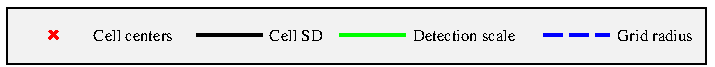
\includegraphics[width=\textwidth]{img/gridType_legend.pdf}
	\end{subfigure}
	\begin{subfigure}[t]{0.32\textwidth}
		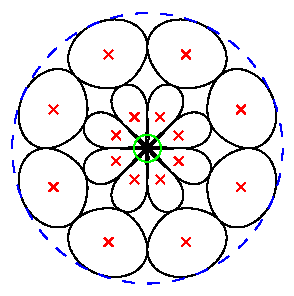
\includegraphics[width=\textwidth]{img/gridType_polar_polar_gaussian.pdf}
		\caption{Polar}
		\label{fig:gridType_ppg}
	\end{subfigure}
	\begin{subfigure}[t]{0.32\textwidth}
		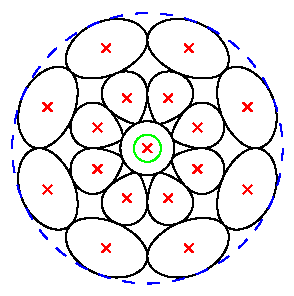
\includegraphics[width=\textwidth]{img/gridType_polar_central_polar_gaussian.pdf}
		\caption{Polar central}
		\label{fig:gridType_pcpg}
	\end{subfigure}
	\begin{subfigure}[t]{0.32\textwidth}
		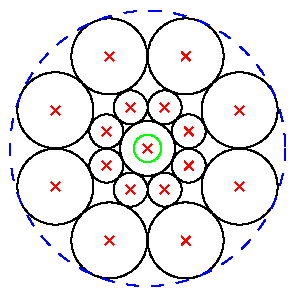
\includegraphics[width=\textwidth]{img/gridType_log-polar.pdf}
		\caption{Log-polar}
		\label{fig:gridType_lp}
	\end{subfigure}
	\begin{subfigure}[t]{0.32\textwidth}
		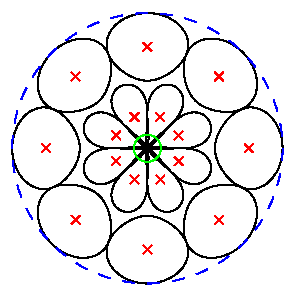
\includegraphics[width=\textwidth]{img/gridType_concentric_polar_polar_gaussian.pdf}
		\caption{Concentric polar}
		\label{fig:gridType_cppg}
	\end{subfigure}
	\begin{subfigure}[t]{0.32\textwidth}
		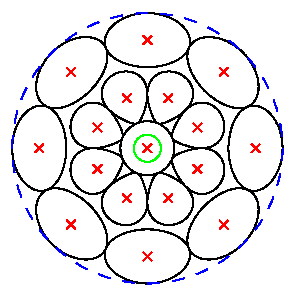
\includegraphics[width=\textwidth]{img/gridType_concentric_polar_central_polar_gaussian.pdf}
		\caption{Concentric polar central}
		\label{fig:gridType_cpcpg}
	\end{subfigure}
	\begin{subfigure}[t]{0.32\textwidth}
		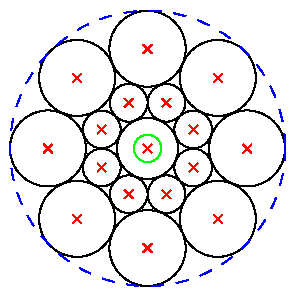
\includegraphics[width=\textwidth]{img/gridType_concentric_log-polar.pdf}
		\caption{Concentric log-polar}
		\label{fig:gridType_clp}
	\end{subfigure}
	\caption{Examples of grid layouts showing cell centers, cell standard deviations, detection scales, and grid radii. The grid size is chosen to be $[8 2]$ (8 cells in each of 2 rings) and the grid radius is set to 10 times detection scale. The polar grids utilize polar Gaussian aperture cell functions while the log-polar use cartesian Gaussian aperture cell functions.}
	\label{fig:gridType}
\end{figure}

Irregular SIFT \cite{cui2009scale}
%
\section{Binning aperture function}
%
\todo{Add reference to section about smooth hisograms/LOI}
The binning aperture function decides the shape of the smooth histograms that make up our descriptor. We define it as a Gaussian function
%
\begin{align}
B(f_i, \x; f) = G(f(\x) - f_i; \sigma)
\end{align}
%
\section{Example}
%
In order to visualize the construction of our descriptor, we will show an example of the whole process. We start by extracting interest points of an image with a multi-scale DoG detector, as shown in \Cref{fig:cellHistDetector}
%
\begin{figure}[H]
    \centering
    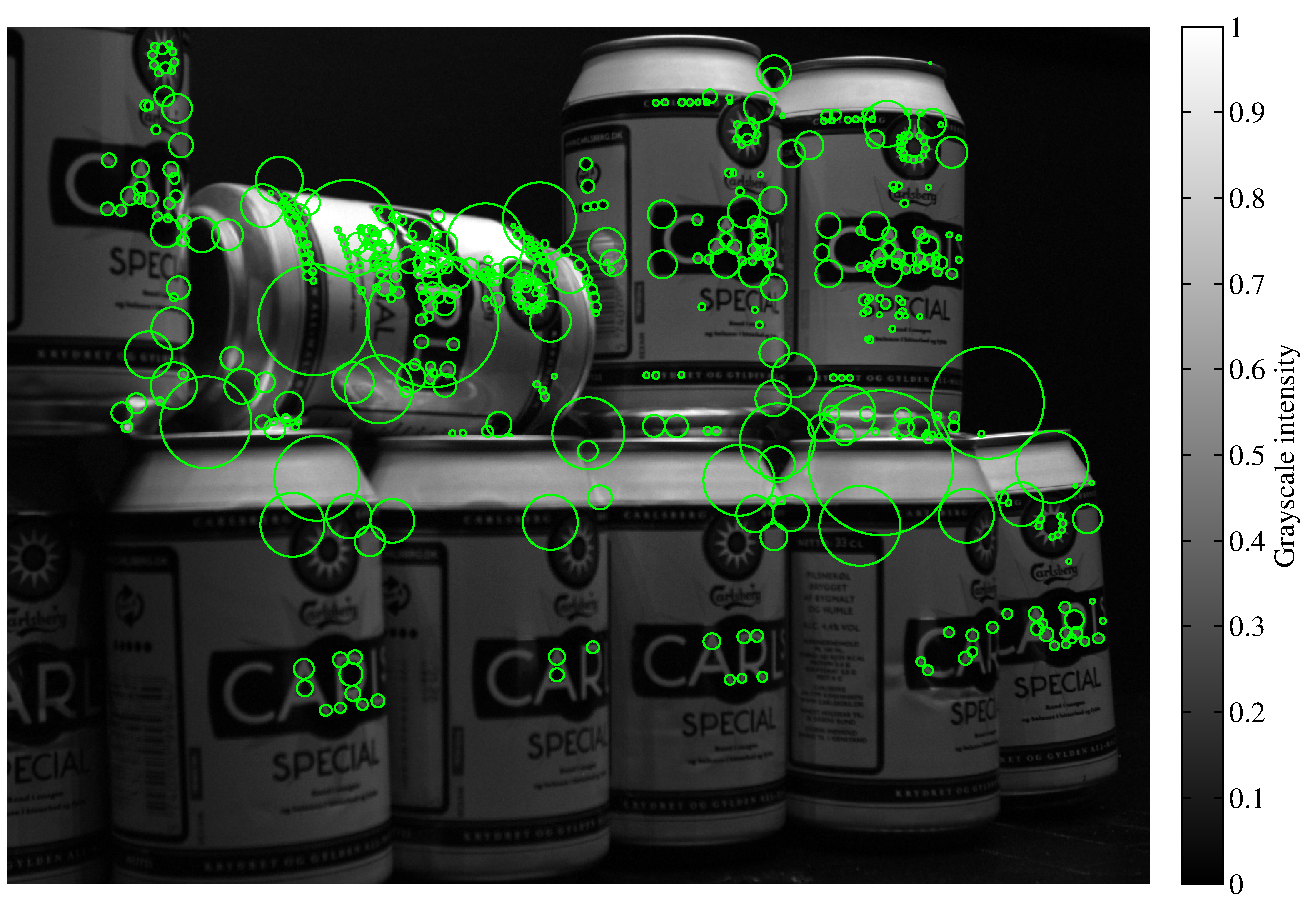
\includegraphics[width=\textwidth]{img/cellHistDetector.pdf}
    \caption{Interest points (in green) found by a multiscale DoG detector on an example image. The size of the circles illustrates the detection scale of each point. $529$ points are detected in total.}
    \label{fig:cellHistDetector}
\end{figure}
%
The next step is to construct the scale space images.
%
\begin{figure}[H]
    \centering
    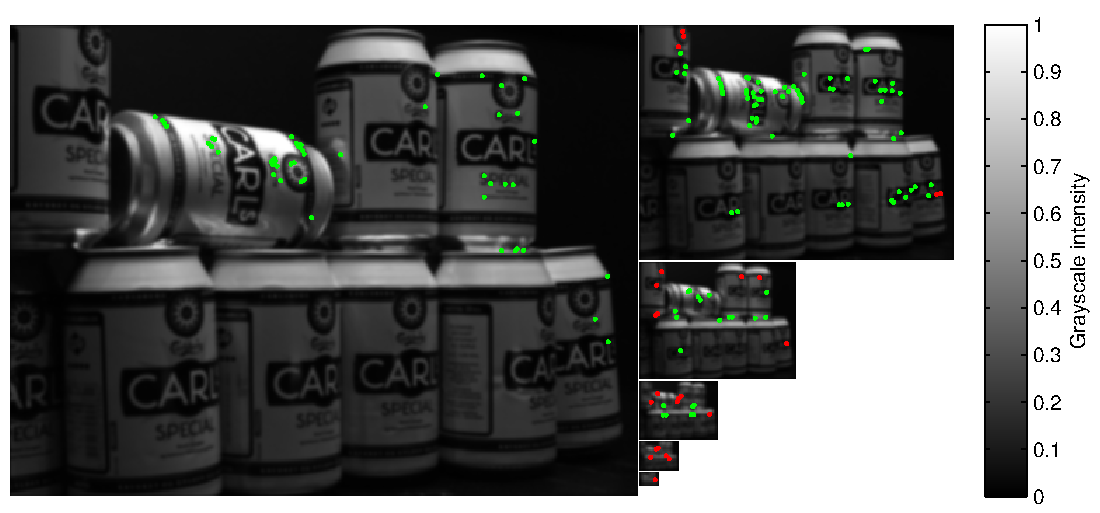
\includegraphics[width=\textwidth]{img/cellHistScaleSpacesP.pdf}
    \caption{}
    \label{fig:cellHistScaleSpacesP}
\end{figure}
%
\begin{figure}[H]
    \centering
    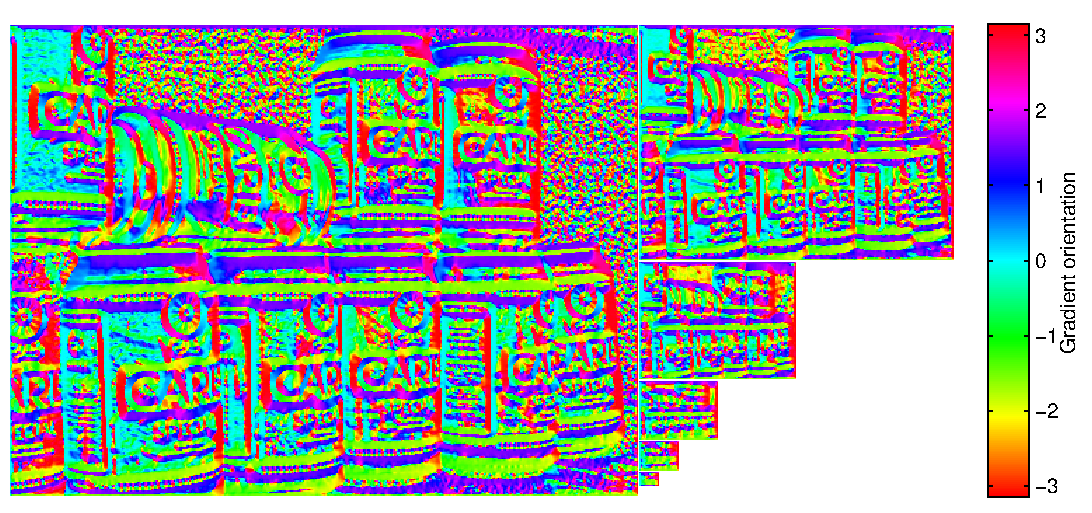
\includegraphics[width=\textwidth]{img/cellHistScaleSpacesV.pdf}
    \caption{}
    \label{fig:cellHistScaleSpacesV}
\end{figure}
%
\begin{figure}[H]
    \centering
    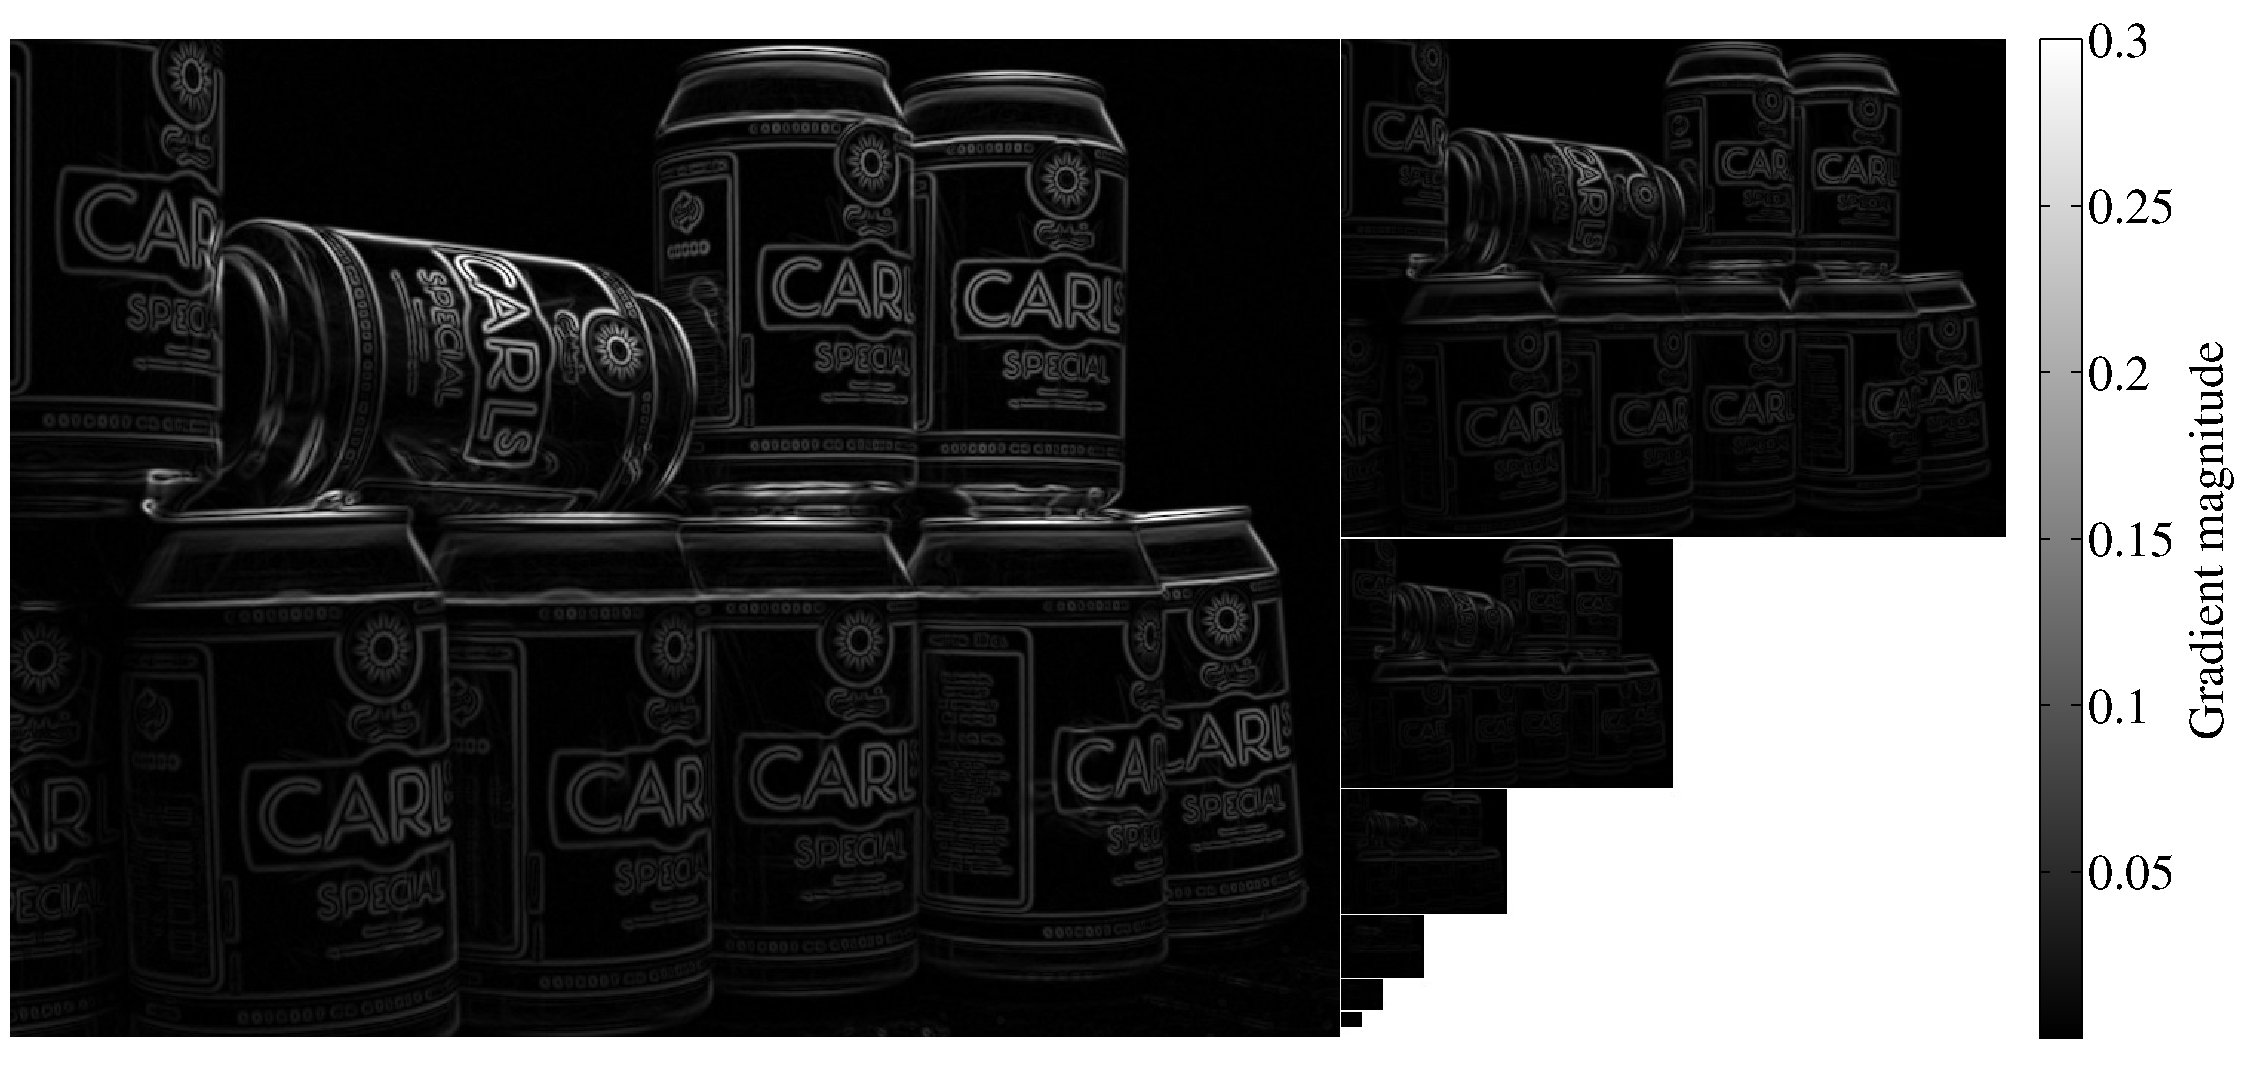
\includegraphics[width=\textwidth]{img/cellHistScaleSpacesM.pdf}
    \caption{}
    \label{fig:cellHistScaleSpacesM}
\end{figure}
%
\begin{figure}[H]
    \centering
    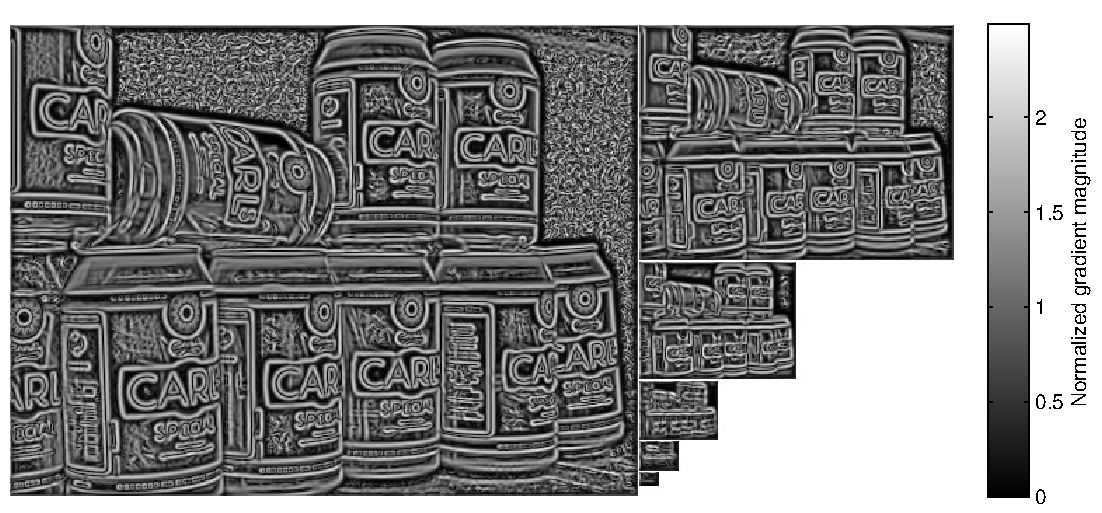
\includegraphics[width=\textwidth]{img/cellHistScaleSpacesMnorm.pdf}
    \caption{}
    \label{fig:cellHistScaleSpacesMnorm}
\end{figure}
%
\begin{figure}[H]
    \centering
    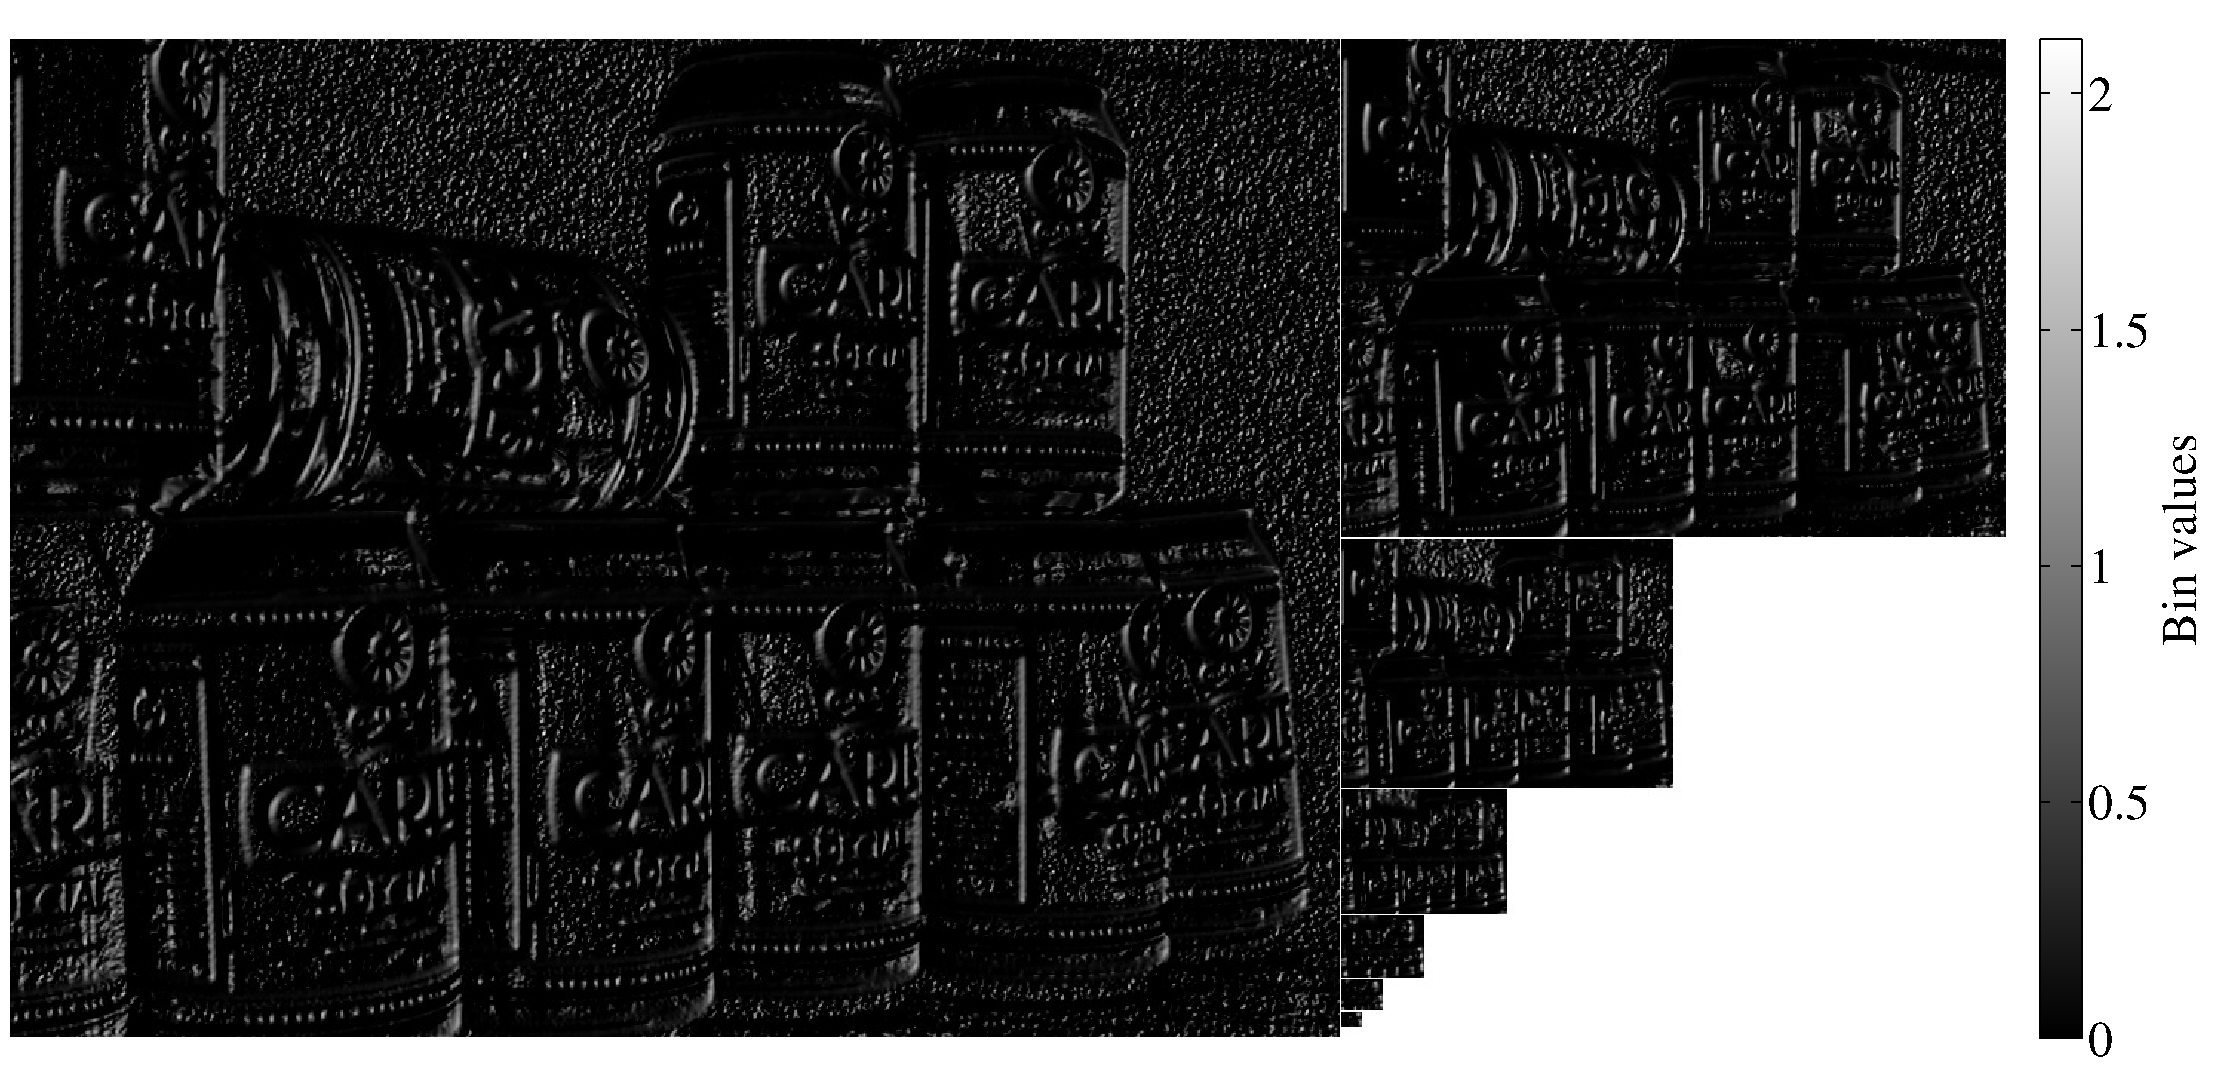
\includegraphics[width=\textwidth]{img/cellHistScaleSpacesBin01.pdf}
    \caption{}
    \label{fig:cellHistScaleSpacesBin01}
\end{figure}
%
\begin{figure}[H]
    \centering
    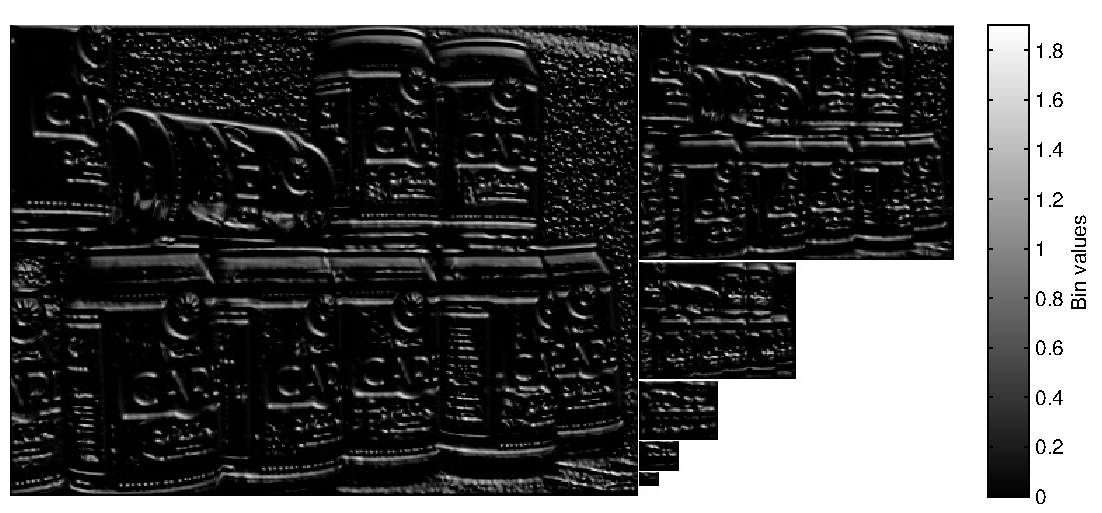
\includegraphics[width=\textwidth]{img/cellHistScaleSpacesBin07.pdf}
    \caption{}
    \label{fig:cellHistScaleSpacesBin07}
\end{figure}
%
\begin{figure}[H]
    \centering
    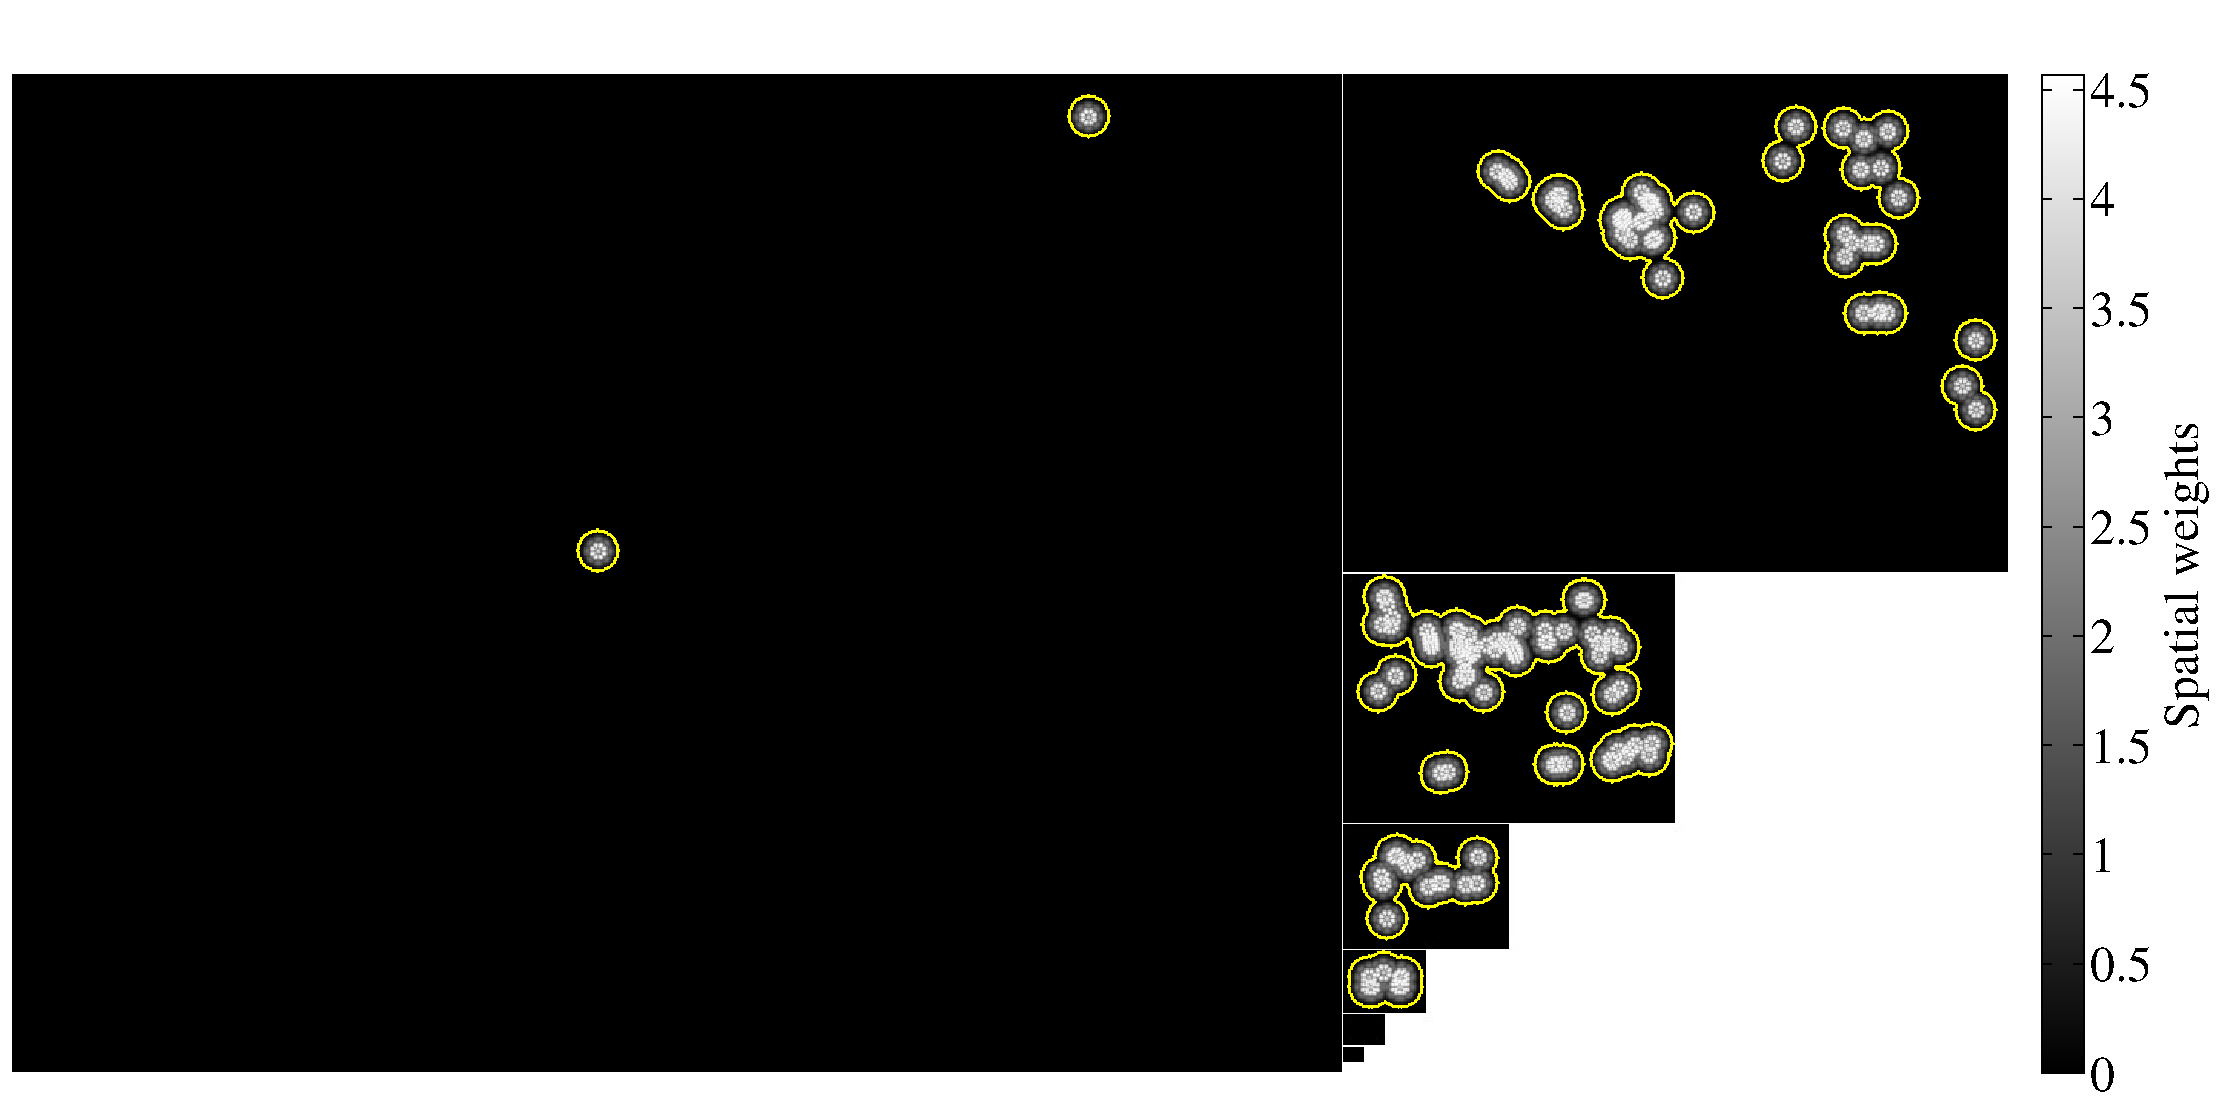
\includegraphics[width=\textwidth]{img/cellHistScaleSpacesSpatialWeights.pdf}
    \caption{}
    \label{fig:cellHistScaleSpacesSpatialWeights}
\end{figure}
%
\section{Notes}
%
% Example scene 47!
%
\begin{enumerate}
%\item Calculate absolute parameters
%\item Approximate scales needed
\item Example of detector output
\item Create scale spaces (approx scales included)
	Implementation: Chain/direct, Gaussian/finite difference
	Figures: Examples of scale space images and their corresponding features
\item Calculate content (gradient orientation, shape index) and magnitudes (gradient magnitude $M$, curvedness $C$)
	Figures: Go, si examples
\item Optional: Pixel normalization of magnitudes
	Figures: Already produced
\item Create cell indices (in scalespaces), remove interest points too close to the edge, compute cell and center weights
	Figures: Removed points, maybe some way of displaying weights
\item Extract magnitudes and values for all image positions inside any cell window
	Figures: intersection and union of cells
\item Compute bin weights and renormalize based on bin area and periodicity
	Figures: 
\item Compute histogram for each cell by multiplying the bin weights, cell weights, magnitudes, and center weights.
\item Optional: Normalize each cell histogram
\item Concatenate cell histograms into feature vectors and normalize
\end{enumerate}
%
\begin{figure}[H]
    \centering
    \begin{subfigure}[t]{0.49\textwidth}
        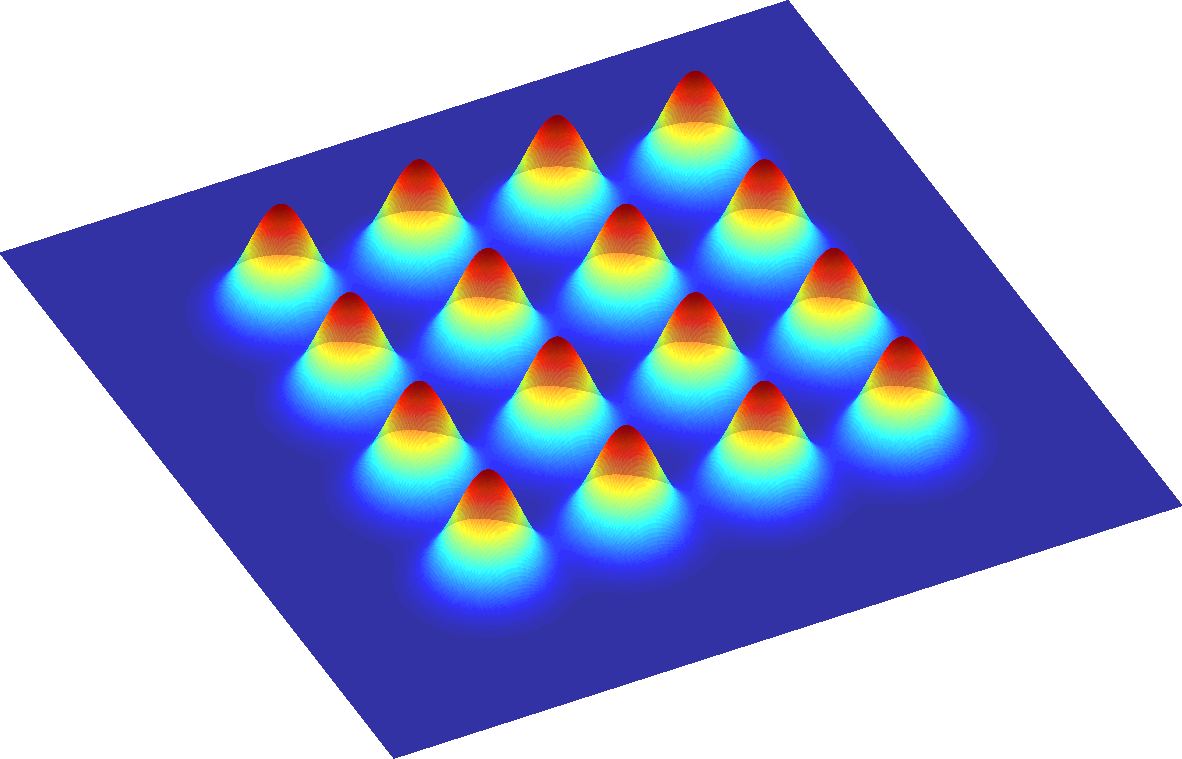
\includegraphics[width=\textwidth]{img/cellLayoutSquare.png}
        \caption{}
        \label{fig:cellLayoutSquare}
    \end{subfigure}
	\begin{subfigure}[t]{0.49\textwidth}
        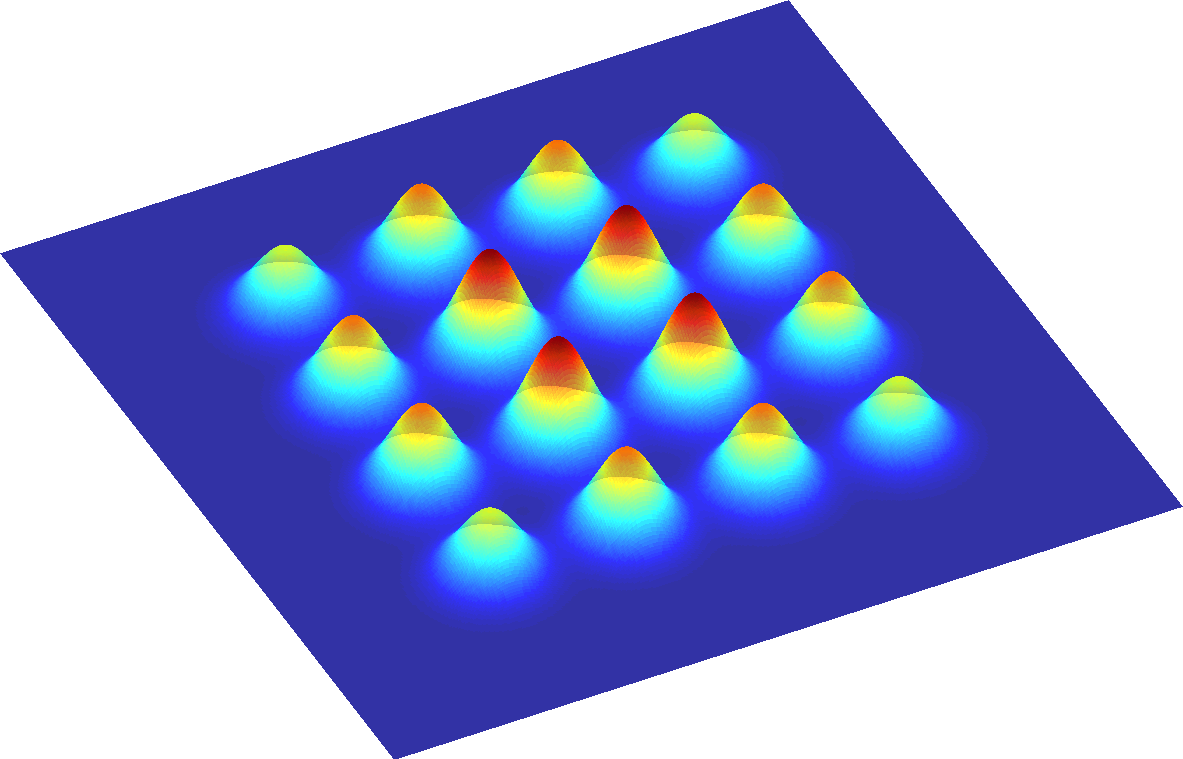
\includegraphics[width=\textwidth]{img/cellLayoutSquareCenter.png}
        \caption{}
        \label{fig:cellLayoutSquareCenter}
    \end{subfigure}
	\begin{subfigure}[t]{0.49\textwidth}
        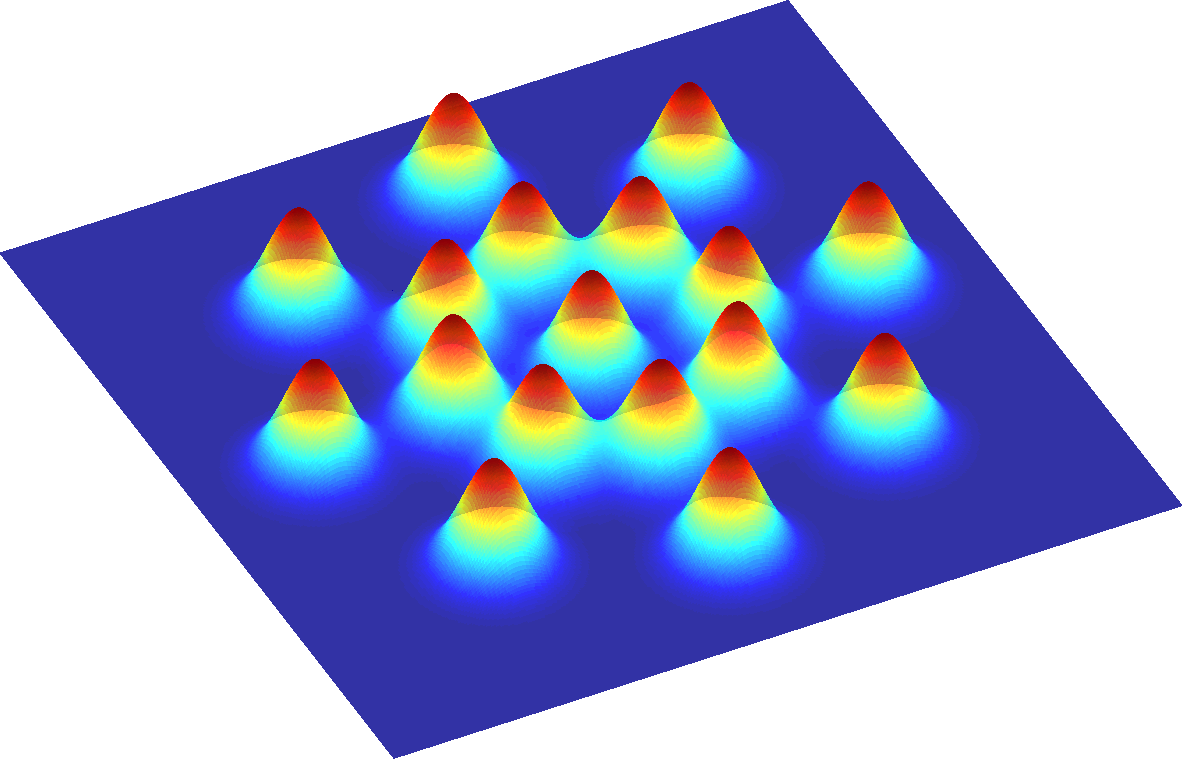
\includegraphics[width=\textwidth]{img/cellLayoutPolar.png}
        \caption{}
        \label{fig:cellLayoutPolar}
    \end{subfigure}
	\begin{subfigure}[t]{0.49\textwidth}
        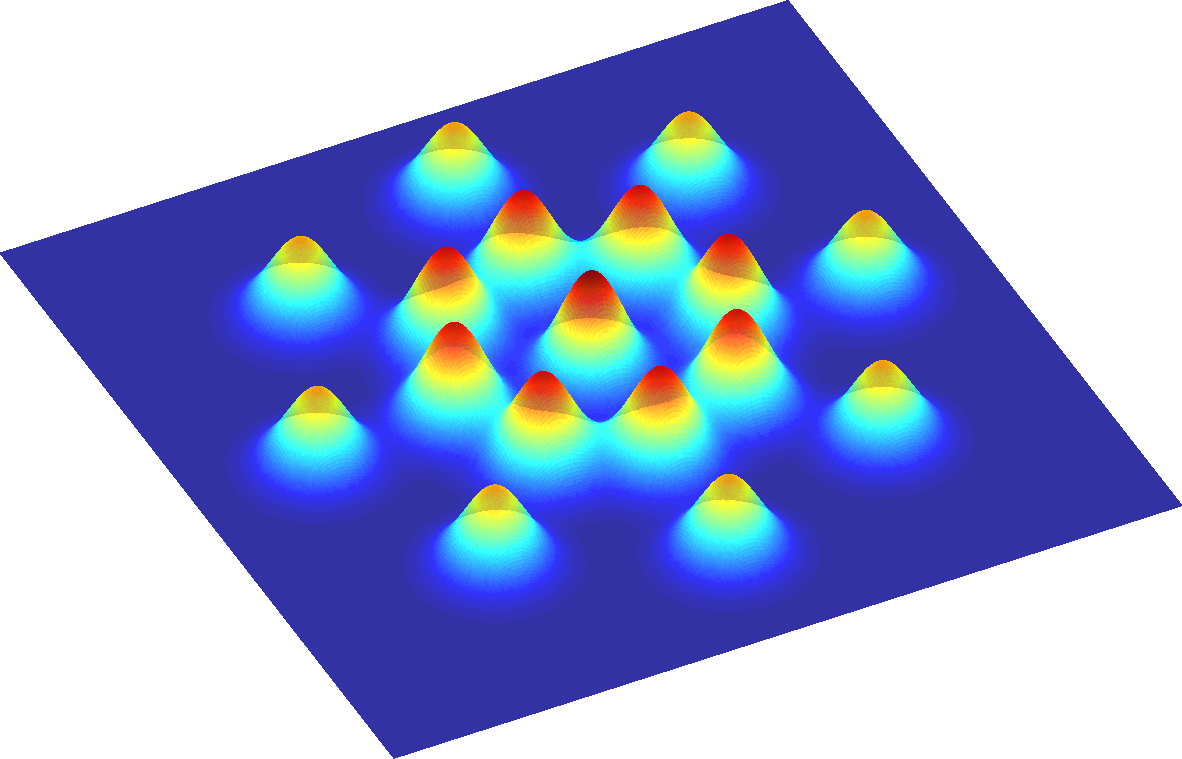
\includegraphics[width=\textwidth]{img/cellLayoutPolarCenter.png}
        \caption{}
        \label{fig:cellLayoutPolarCenter}
    \end{subfigure}
	\begin{subfigure}[t]{0.49\textwidth}
        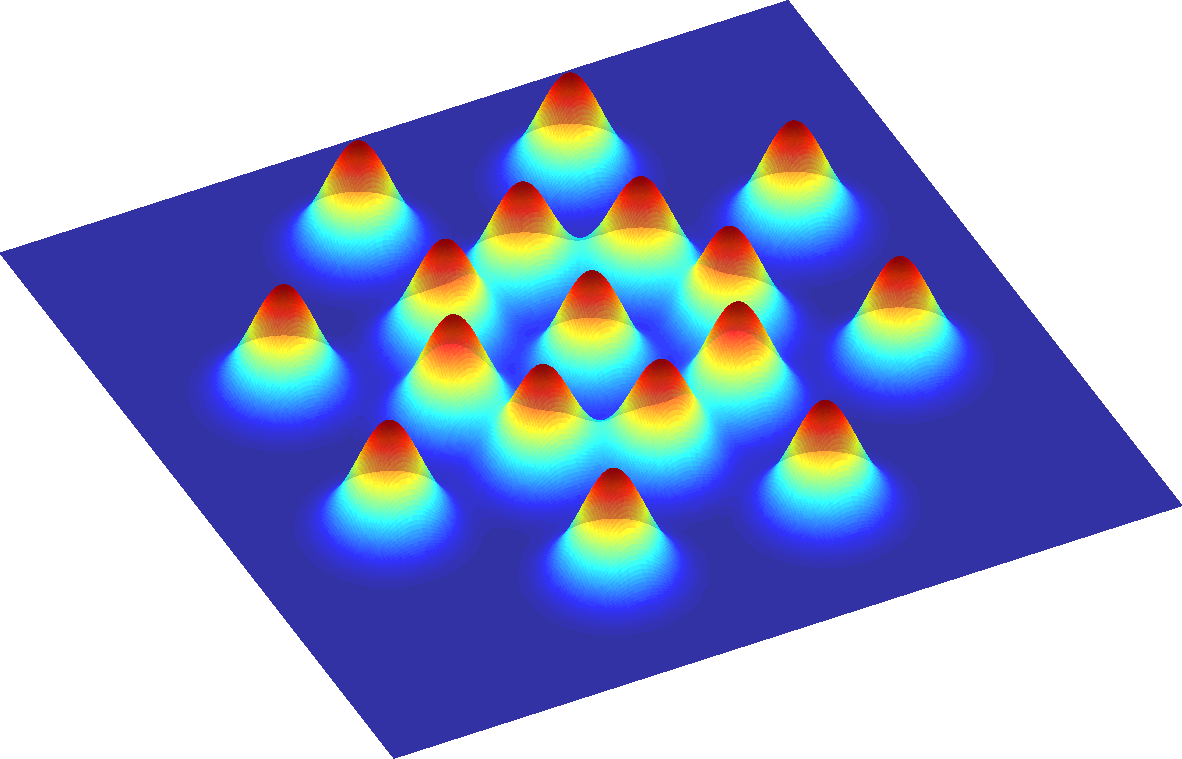
\includegraphics[width=\textwidth]{img/cellLayoutConcentricPolar.png}
        \caption{}
        \label{fig:cellLayoutConcentricPolar}
    \end{subfigure}
	\begin{subfigure}[t]{0.49\textwidth}
        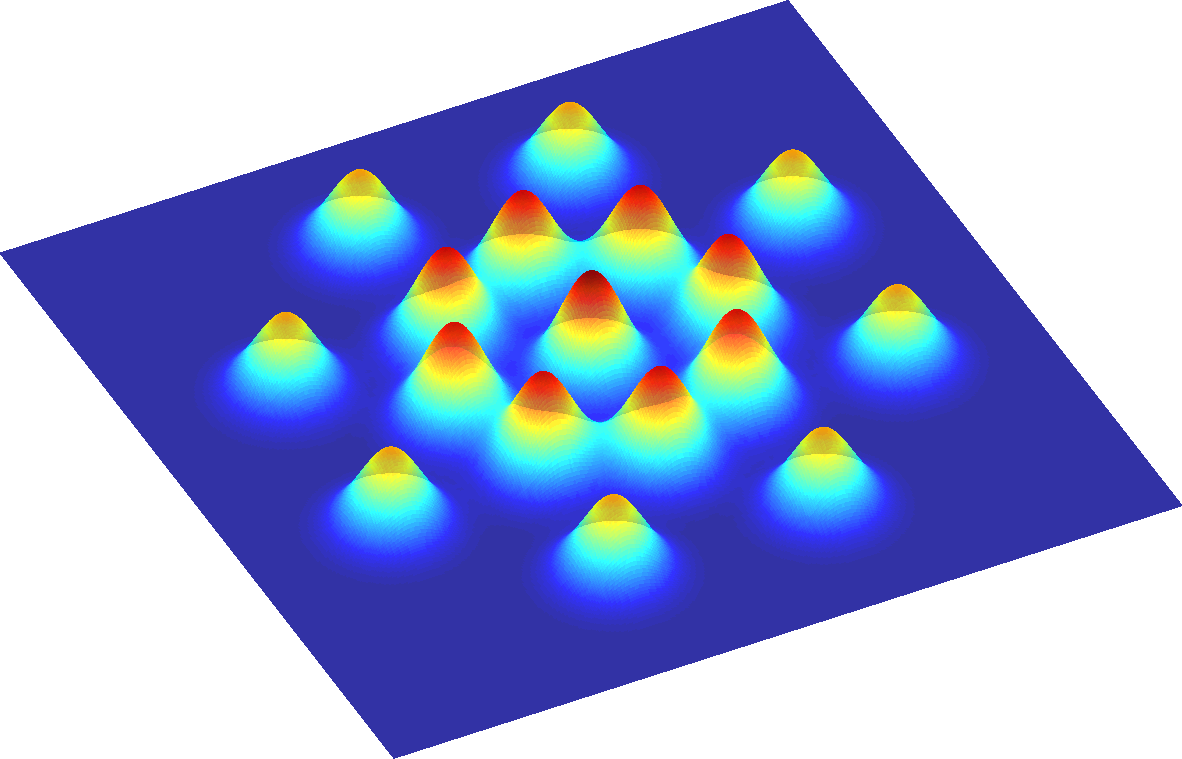
\includegraphics[width=\textwidth]{img/cellLayoutConcentricPolarCenter.png}
        \caption{}
        \label{fig:cellLayoutConcentricPolarCenter}
    \end{subfigure}
    \caption{}
\end{figure}
%
\begin{figure}[H]
    \centering
    \begin{subfigure}[t]{0.49\textwidth}
        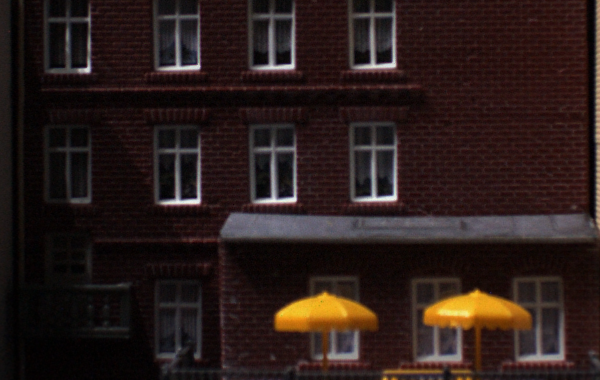
\includegraphics[width=\textwidth]{img/pixelNormalizationExample1.png}
        \caption{}
        \label{fig:pixelNormalizationExample1}
    \end{subfigure}
    \begin{subfigure}[t]{0.49\textwidth}
        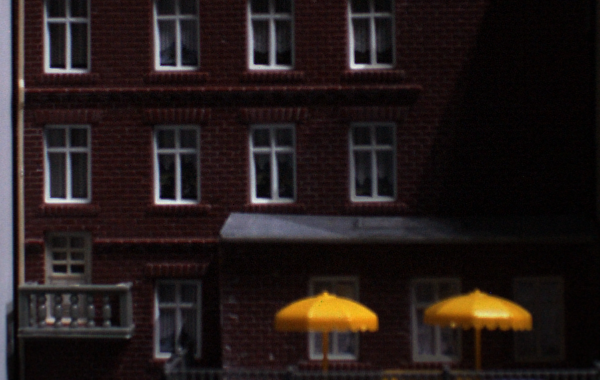
\includegraphics[width=\textwidth]{img/pixelNormalizationExample2.png}
        \caption{}
        \label{fig:pixelNormalizationExample2}
    \end{subfigure}
    \begin{subfigure}[t]{0.49\textwidth}
        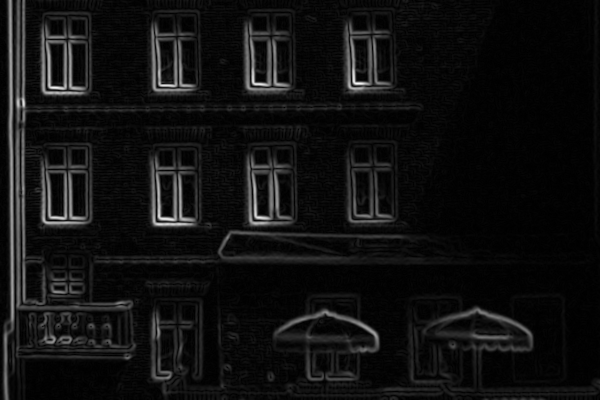
\includegraphics[width=\textwidth]{img/pixelNormalizationExample3.png}
        \caption{}
        \label{fig:pixelNormalizationExample3}
    \end{subfigure}
    \begin{subfigure}[t]{0.49\textwidth}
        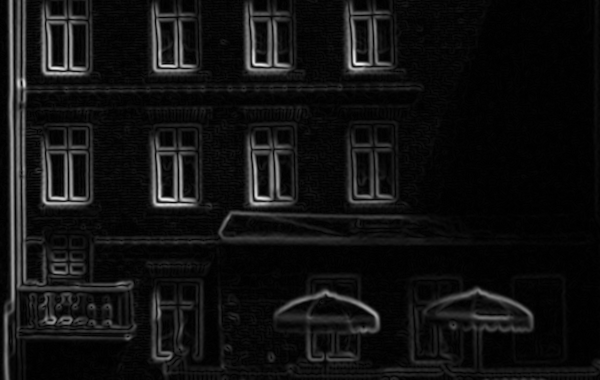
\includegraphics[width=\textwidth]{img/pixelNormalizationExample4.png}
        \caption{}
        \label{fig:pixelNormalizationExample4}
    \end{subfigure}
    \begin{subfigure}[t]{0.49\textwidth}
        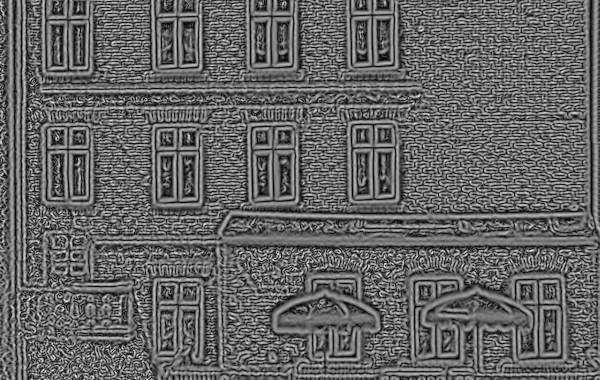
\includegraphics[width=\textwidth]{img/pixelNormalizationExample5.png}
        \caption{}
        \label{fig:pixelNormalizationExample5}
    \end{subfigure}
    \begin{subfigure}[t]{0.49\textwidth}
        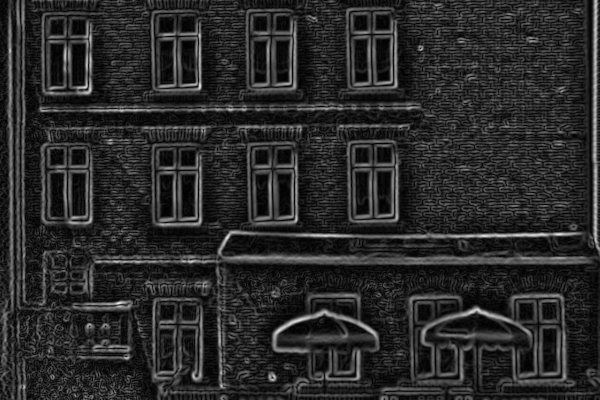
\includegraphics[width=\textwidth]{img/pixelNormalizationExample6.png}
        \caption{}
        \label{fig:pixelNormalizationExample6}
    \end{subfigure}
    \begin{subfigure}[t]{0.49\textwidth}
        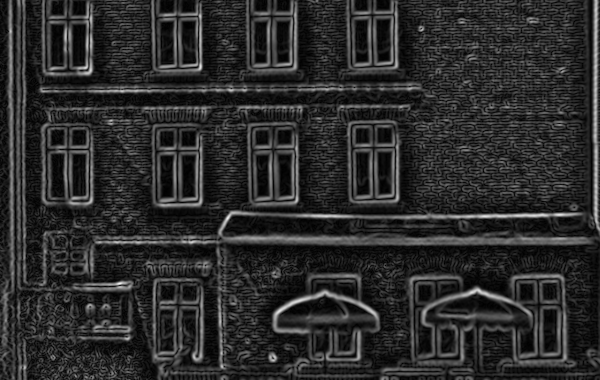
\includegraphics[width=\textwidth]{img/pixelNormalizationExample7.png}
        \caption{}
        \label{fig:pixelNormalizationExample7}
    \end{subfigure}
    \begin{subfigure}[t]{0.49\textwidth}
        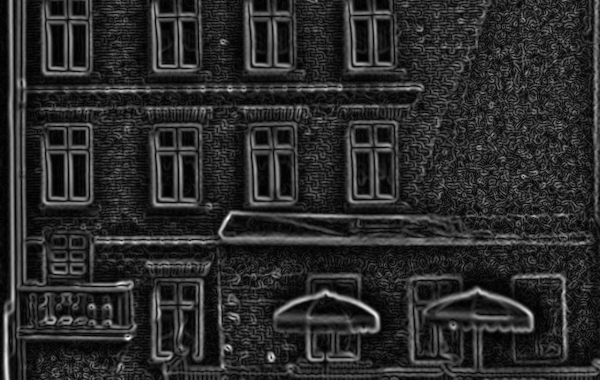
\includegraphics[width=\textwidth]{img/pixelNormalizationExample8.png}
        \caption{}
        \label{fig:pixelNormalizationExample8}
    \end{subfigure}
    \caption{Images \subref{fig:pixelNormalizationExample1} and \subref{fig:pixelNormalizationExample2} show cut-outs of an image with leftmost and rightmost artificial lighting, respectively. Images \subref{fig:pixelNormalizationExample3} and \subref{fig:pixelNormalizationExample4} show gradient magnitudes of these images. Images \subref{fig:pixelNormalizationExample5} and \subref{fig:pixelNormalizationExample6} show pixel normalized magnitudes for $\sigma_\text{norm} = 2$. Images \subref{fig:pixelNormalizationExample7} and \subref{fig:pixelNormalizationExample8} show pixel normalized magnitudes for $\sigma_\text{norm} = 10$.}
    \label{fig:pixelNormalizationExample}
\end{figure}
%
\subsection{Histogram normalization}

- No cell normalization -> Center (cell)

0. Center (pixels) -> no normalization
1. Center (pixels) -> cell normalization
2. Center (pixels) -> Cell normalization -> Center (cell)
3. Cell normalization -> Center (cell)

Center (cell)


\subbibliography

\end{document}
